\documentclass[../main.tex]{subfiles}

\begin{document}

\chapter{Background}

\section{Containerization} 

A \textbf{container} is a standardized software unit that packages code and its dependencies, ensuring the application runs consistently across different environments. According to the 2024 Stack Overflow Developer Survey \cite{surveystackoverflow}, Docker is the most widely used tool among professional developers, with 59\% adoption. Docker is an open platform for developing, shipping, and running applications, enabling containerization and deployment across various environments. A Docker \textbf{container image} is a lightweight, standalone package that includes everything needed to execute an application, such as code, runtime, system tools, libraries, and settings. At runtime, container images become active containers. \cite{container}

While Docker containers simplify application packaging and deployment, Kubernetes extends this by providing orchestration, automation, and scalability for managing containerized applications across multiple environments. Kubernetes is an open-source platform, originally designed by Google, first released in 2015.

\begin{figure}[H]
    \centering
    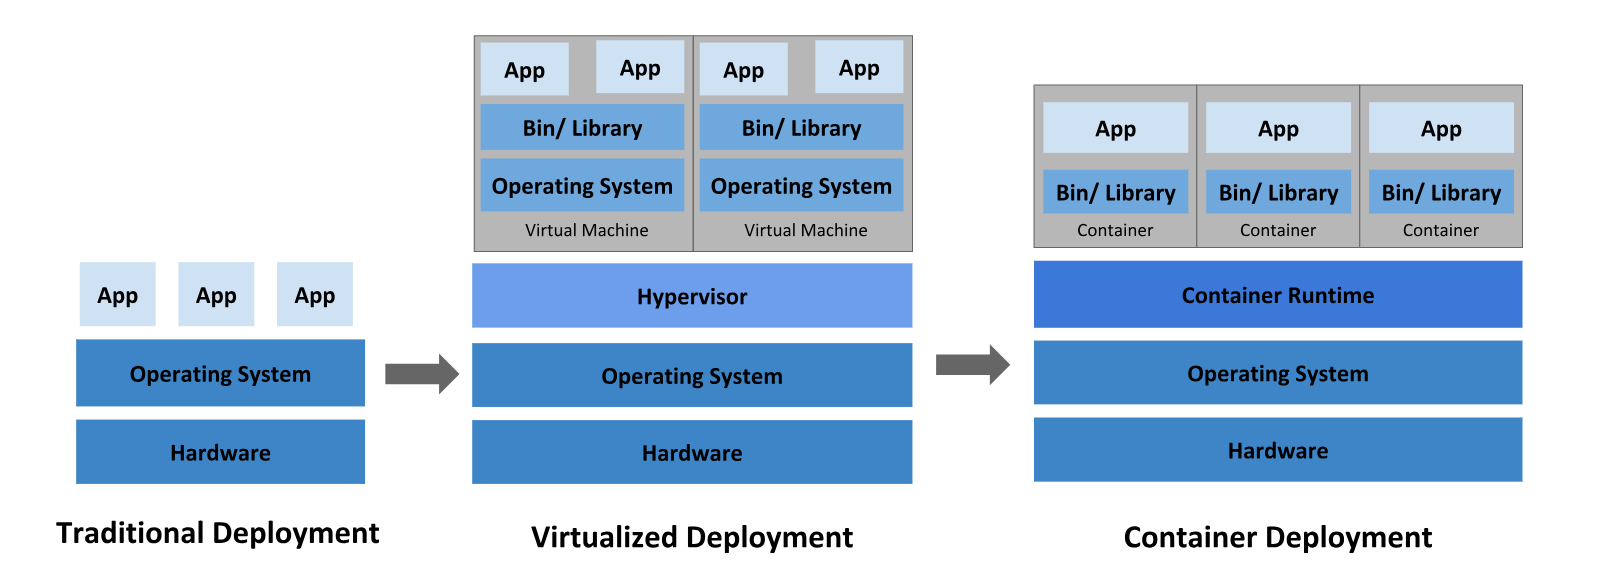
\includegraphics[scale=0.5]{img/3-background/kubernetes/container_evolution.png}
    \caption{Container Evolution. \protect\footnotemark}
    \label{fig:container_evolution}
\end{figure}

\footnotetext{\url{Source: https://kubernetes.io/images/docs/Container\_Evolution.svg (accessed: 18.03.2025)}}


Figure \ref{fig:container_evolution} depicts the progression of deployment methods, from traditional physical servers to virtual machines (VMs) and, ultimately, containerized environments. Initially, applications operated directly on physical servers, which often led to challenges in resource allocation and higher operational costs. The introduction of virtualization addressed these issues by enabling multiple VMs to run on a single server, improving resource utilization, scalability, and security. Containers further enhanced deployment efficiency by allowing applications to share the host operating system while maintaining isolation. Due to their lightweight and portable nature, containers have become well-suited for cloud environments. Kubernetes plays a key role in managing these containerized applications by providing a structured framework for deployment and operation. \cite{kubernetes}

\section{Kubernetes Architecture}

 A Kubernetes cluster is composed of a control plane and a group of worker machines, known as nodes, which execute containerized applications. Each cluster requires at least one worker node to run Pods. The figure \ref{fig:components} presents a high-level overview of the key components that form a Kubernetes cluster. It illustrates the control plane, which manages the cluster's state, and the worker nodes, which run containerized applications. \cite{kubernetes}
 
\begin{figure}[H]
    \centering
    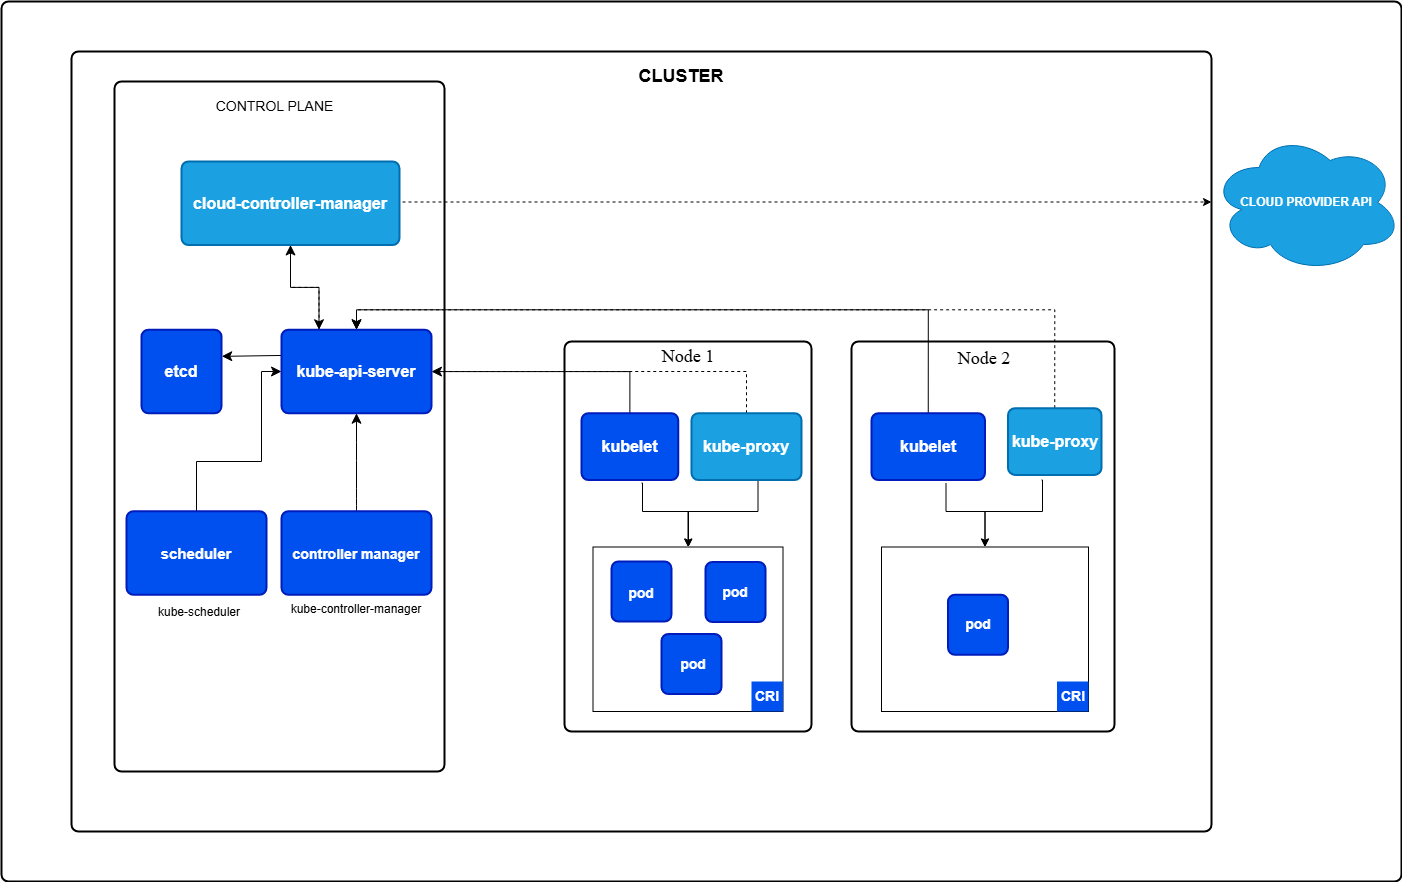
\includegraphics[scale=0.3]{img/3-background/kubernetes/components.png}
    \caption{A high-level overview of the essential components that make up a Kubernetes cluster. \protect\footnotemark}
    \label{fig:components}
\end{figure}

\footnotetext{Source: https://kubernetes.io/images/docs/kubernetes-cluster-architecture.svg (accessed 10.03.2025)}

\textbf{Control Plane}: The control plane manages the overall state of the cluster and includes the following components:  

\begin{enumerate}
    \item[] kube-apiserver – The core component that exposes the Kubernetes HTTP API.
    \item[] etcd – A highly available and consistent key-value store for all API server data.  
    \item[] kube-scheduler – Assigns unbound Pods to suitable nodes.  
    \item[] kube-controller-manager – Runs controllers to enforce Kubernetes API behavior.  
    \item[] cloud-controller-manager (optional) – Integrates Kubernetes with cloud providers.  
\end{enumerate}

\textbf{Node Plane}: Each node runs components responsible for maintaining running Pods and providing the Kubernetes runtime environment.

\begin{enumerate}
    \item[] kubelet – Ensures Pods and their containers are running.  
    \item[] kube-proxy (optional) – Manages network rules to implement Services.  
    \item[] Container runtime (CRI) – Executes containers within the node.
\end{enumerate}

\section{Helm}

Helm is a package manager for Kubernetes that simplifies the definition, installation, and management of complex applications using Helm Charts. Helm charts are publicly available on Artifact Hub website. \cite{helm} 

Helm allows users to create, package, and manage Helm charts. It enables storing and retrieving charts from repositories, installing, upgrading, and uninstalling Kubernetes applications, and managing application release cycles. Helm is written in the Go programming language. It uses the Kubernetes client library via REST+JSON and stores data in Kubernetes Secrets without requiring an external database. Configuration files are written in YAML where possible. A chart is a package containing Kubernetes application definitions. A config consists of configuration settings applied to a chart. A release is a deployed instance of a chart with a specific configuration. The Helm Client is a command-line tool that allows users to manage charts, repositories, and releases. The Helm Library executes Helm operations, interacts with the Kubernetes API, and handles installation, upgrades, and uninstallation. \cite{helmarchitecture}

\section{Rancher}

Rancher is a Kubernetes management platform that enables cluster deployment across any infrastructure. It supports multiple provisioning methods, including hosted providers, on-premise setups, and importing existing clusters. 

Beyond deployment, Rancher offers centralized authentication, role-based access control (RBAC), monitoring, alerting, and integration with external logging tools. It also supports Helm-based application deployment and includes Fleet, a built-in GitOps solution for automating workload management. \cite{rancher}

Rancher provides a user-friendly interface that simplifies application workload management. It is designed to be accessible for those with limited Kubernetes expertise.

The figure below illustrates Rancher’s role in IT and DevOps environments. Development teams deploy applications on their chosen public or private cloud platforms, while IT-administrators oversee operations, enforce policies, and maintain visibility across users, clusters, and cloud infrastructure.

\begin{figure}[H]
    \centering
    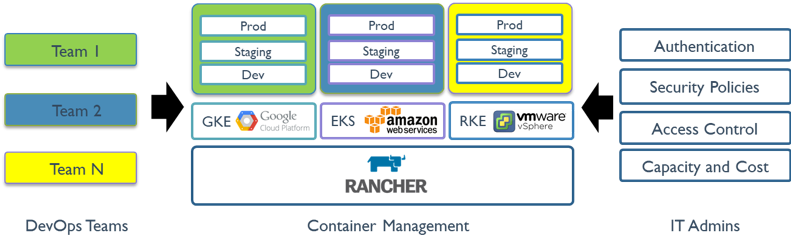
\includegraphics[scale=0.5]{img/3-background/rancher/rancher_devops_teams.png}
    \caption{Rancher’s Role Between DevOps Teams and IT Administrators. \protect\footnotemark}
    \label{fig:rancher_devops_teams}
\end{figure}

\footnotetext{Source: https://ranchermanager.docs.rancher.com/assets/images/platform-9c0c4130a7a0828898dbc7af56f76df7.png (accessed: 19.03.2025)}

Rancher \gls{cli} is available as a tool to interact with Rancher on a local work station along with the \gls{ui}. The Rancher interface provides access to all management and configuration tools available in Rancher. It offers greater functionality than the \gls{cli} and is the only method for installing dashboard applications or Rancher feature charts.

\begin{figure}[H]
    \centering
    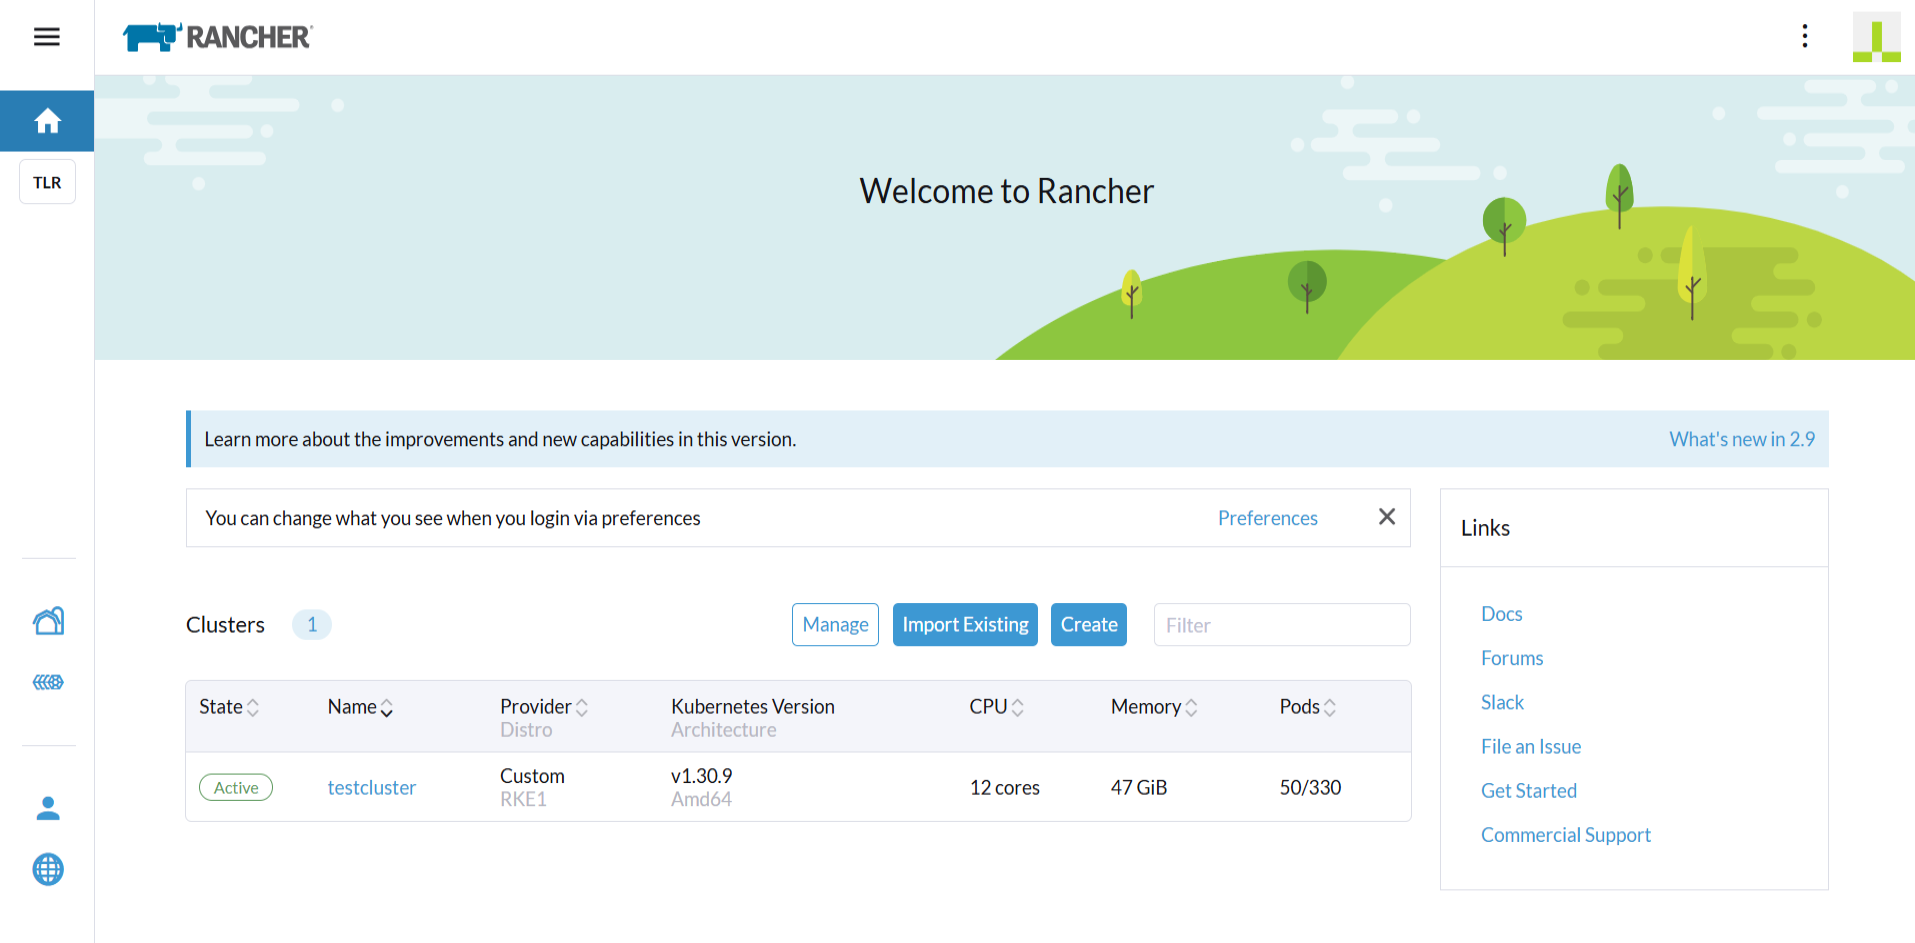
\includegraphics[scale=0.4]{img/3-background/rancher/rancher-gui.png}
    \caption{Rancher’s main page of the \texttt{"testcluster"} on the company's premises.}
    \label{fig:rancher_gui}
\end{figure}

Figure \ref{fig:rancher_gui} displays the main page of the RKE1 cluster \texttt{"testcluster"} in a running state. Figure \ref{fig:rancher_gui_apps} highlights the available menu options and the Apps/Charts section, showcasing the Helm charts that can be installed on the cluster with a single click.
%what is RKE1?
\begin{figure}[H]
    \centering
    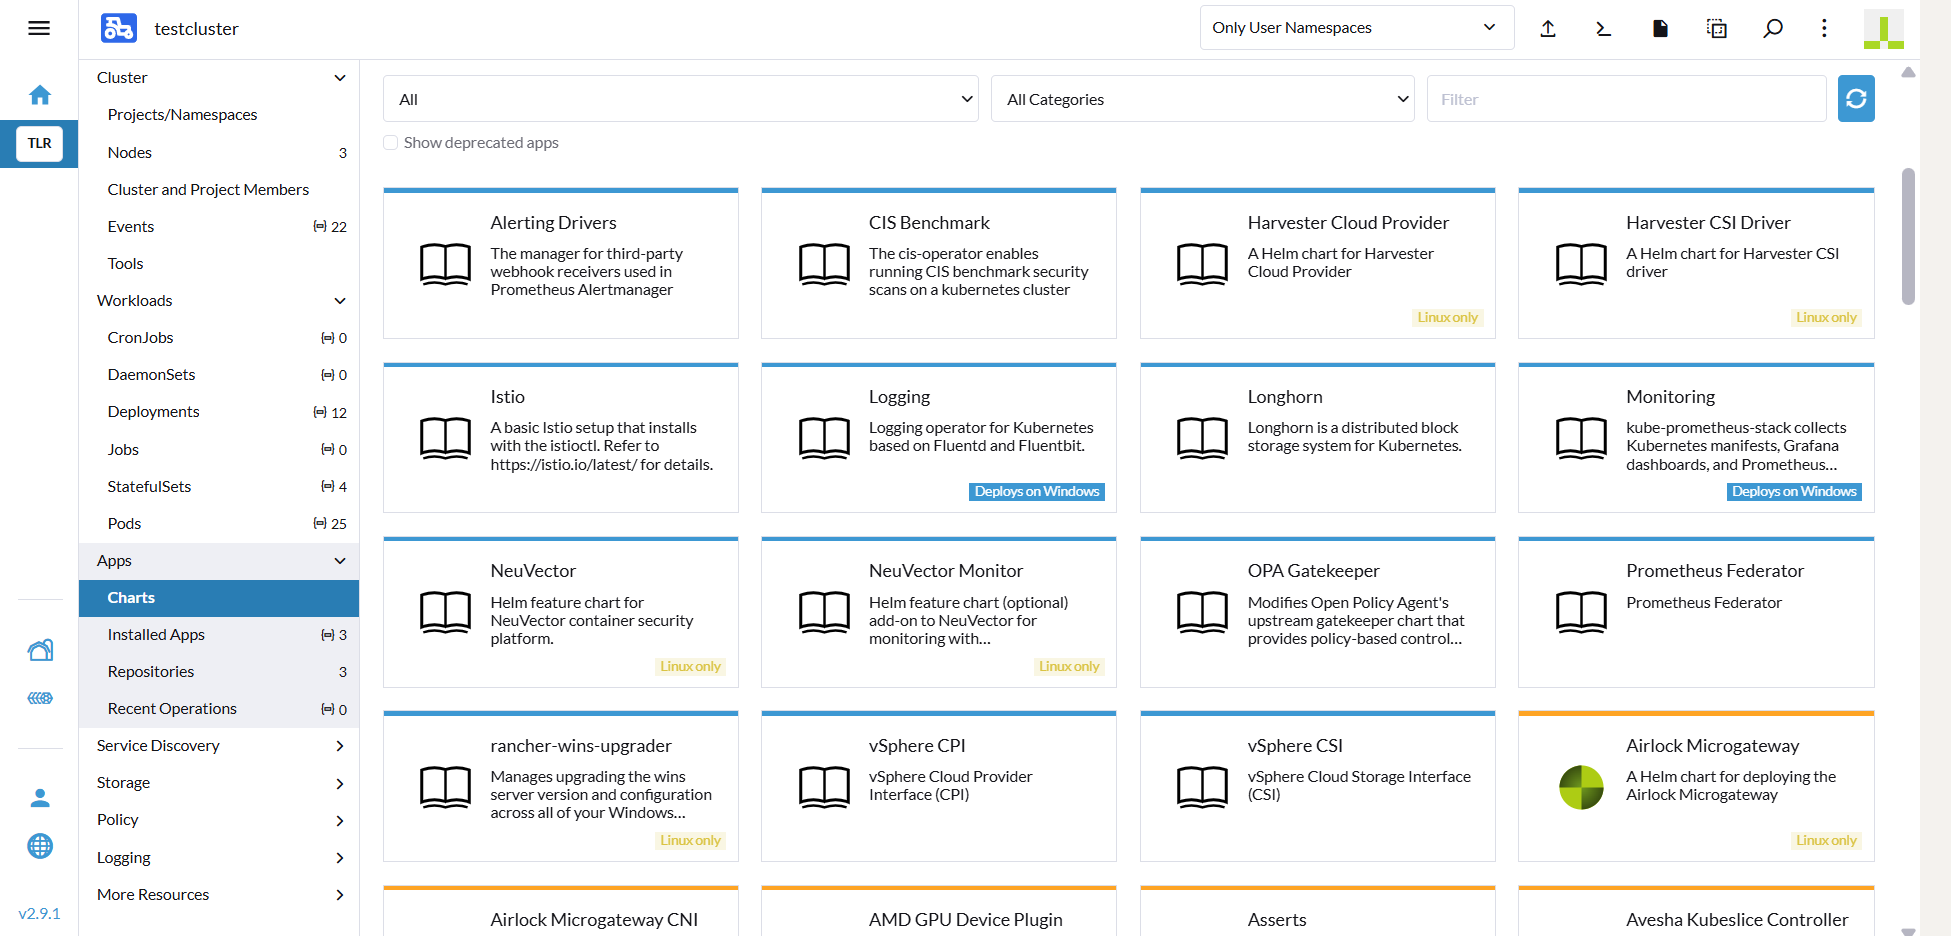
\includegraphics[scale=0.4]{img/3-background/rancher/rancher_gui_apps.png}
    \caption{Rancher’s page under Apps/Charts of the \texttt{"testcluster"} on the company's premise.}
    \label{fig:rancher_gui_apps}
\end{figure}

\textbf{Rancher Architecture}

Figure \ref{fig:rancher_users} illustrates the Rancher architecture, assuming Rancher is managing an RKE2 cluster \texttt{"User Cluster 1"} and a K3s cluster \texttt{"User Cluster 2"}.
%what about RKE1 is it also from Kubernetes?
RKE2 is Rancher's enterprise-ready Kubernetes distribution, designed for security, stability, and compliance \cite{rke2}. K3s is a lightweight Kubernetes version, optimized for resource efficiency and edge computing environments \cite{K3s}.

\begin{figure}[H]
    \centering
    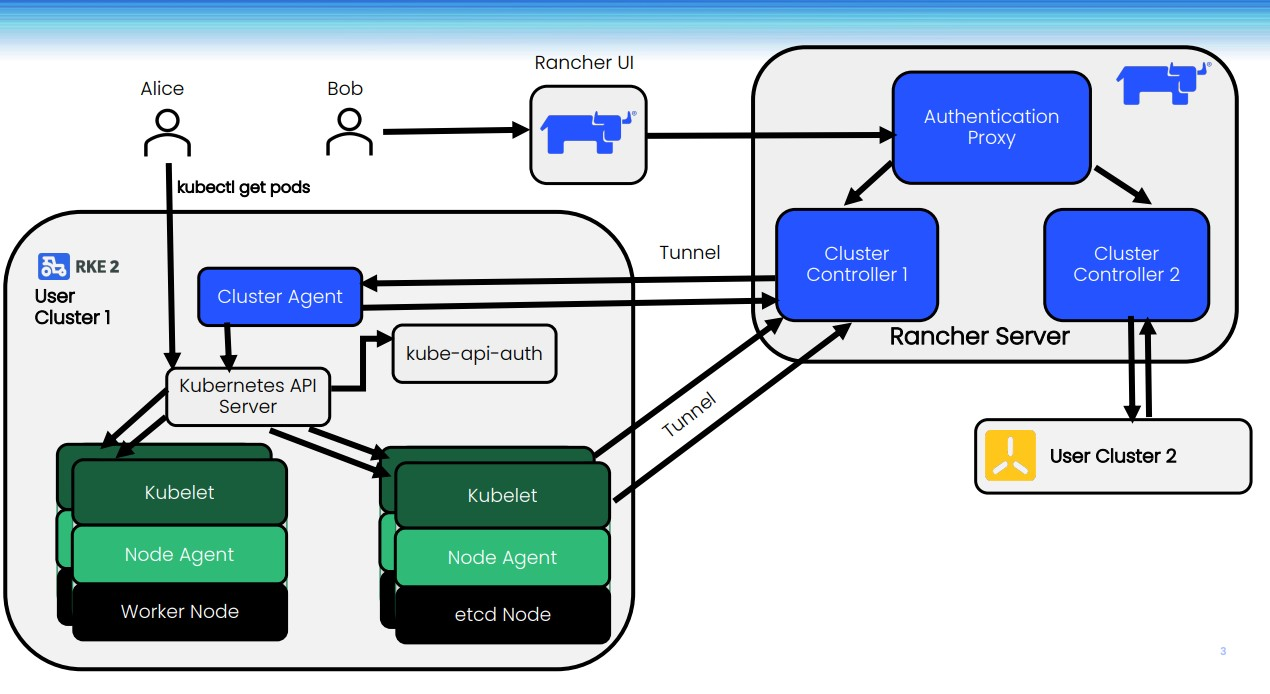
\includegraphics[scale=0.3]{img/3-background/rancher/rancher_users.png}
    \caption{Rancher Users. \protect\footnotemark}
    \label{fig:rancher_users}
\end{figure}

\footnotetext{Source: https://www.rancher.academy/courses/take/rancher-basics/lessons/42838206-the-rancher-architecture-lesson (accessed 10.12.2024)}

Assume there are two users: IT-administrator Bob and developer Alice. Bob requires access to all clusters, while Alice only needs access to the RKE2 cluster.

For every Kubernetes API call, the Authentication Proxy in the Rancher Server sets the appropriate impersonation headers and forwards the request to the control plane of the respective Kubernetes cluster via a tunnel. This tunnel is managed by the Cluster Agent, which runs on every downstream cluster and connects to the corresponding Cluster Controller residing on the Rancher Management Servers. 

Each Cluster Controller is responsible for:

\begin{enumerate}
    \item Monitoring resource changes in downstream clusters.
    \item Reconciling the cluster state to match the desired configuration.
    \item Configuring access control policies for clusters and projects.
    \item Provisioning clusters by invoking the necessary machine drivers and Kubernetes engines.
\end{enumerate}

If the Cluster Agent becomes unavailable in a cluster, the Node Agent — deployed as a DaemonSet on every worker node—takes over tunneling responsibilities.  

The Node Agent is typically responsible for:

\begin{enumerate}
    \item Performing cluster-wide operations, such as Kubernetes version upgrades.
    \item Creating and restoring RKE snapshots. 
\end{enumerate}
% Explain that this is what you are doing for your thesis and that this explains the direct arrow Alice -> RKE2
Alice and Bob can access the RKE2 cluster via the Rancher \gls{ui} or \gls{cli} using Authorized Cluster Endpoint to perform necessary operations.  

When Rancher provisions Kubernetes using RKE/RKE2, an Authorized Cluster Endpoint can be configured. This enables a direct connection to the Kubernetes API of the downstream cluster, bypassing the Authentication Proxy. When enabled, Rancher generates additional Kubernetes API endpoints in the kubeconfig file, allowing direct cluster access. This file includes credentials for both kubectl and Helm. The Authorized Cluster Endpoint is not available for imported clusters or clusters in hosted Kubernetes providers (e.g., Amazon EKS).
The Authorized Cluster Endpoint ensures continuous access to Rancher-managed clusters, e.g. during planned downtime of the Rancher Management Server or during an unplanned outage. Once Rancher is restored, changes made during downtime will be synchronized through the existing tunneling mechanism.

Every user is authenticated against the Rancher Authentication Proxy, based on their assigned global permissions and roles. Permissions determine who can access a given resource. Roles define what actions a user can perform on those resources. This model ensures fine-grained access control across multiple clusters. \cite{rancherbasics}

\section{Kubernetes Logging Architecture}

Containerized applications generate logs by writing to standard output (`stdout`) and standard error (`stderr`) streams. While container engines provide basic logging support, they are not a complete logging solution. Kubernetes itself does not include a built-in storage solution for log data, but external logging systems can be integrated. However, if a container crashes or a node fails, application logs will be lost. \cite{loggingkubernetes}

\begin{figure}[H]
    \centering
    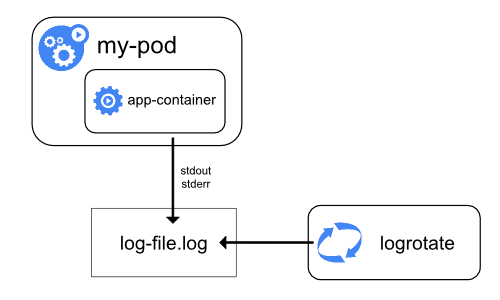
\includegraphics[scale=0.5]{img/3-background/kubernetes/k8s_logs.png}
    \caption{Container logs in Kubernetes. \protect\footnotemark}
    \label{fig:k8_logs}
\end{figure}

\footnotetext{Source: https://kubernetes.io/images/docs/user-guide/logging/logging-node-level.png (accessed 10.03.2025}

\section{Containerized Application Logging}
Containerized applications write logs to standard output (\texttt{stdout}) and standard error (\texttt{stderr}) streams. While container engines support logging, they are not a complete logging solution.  
Kubernetes does not provide a built-in storage mechanism for log data; however, it allows integration with external logging solutions. If a container crashes or a node fails, the associated application logs are lost.

\section{Node-Level Logging}
A container runtime manages and redirects any output generated by a containerized application's \texttt{stdout} and \texttt{stderr} streams.  
The \texttt{kubelet} makes logs accessible through the Kubernetes API. The primary method for retrieving logs is using the \texttt{kubectl logs} command. When executed, the \texttt{kubelet} on the respective node processes the request and returns the log file contents.

Kubernetes also supports log rotation through \texttt{kubelet}, which rotates logs based on predefined configurations.

\section{System Component Logs}
System components in Kubernetes can be classified into two types:  
\begin{itemize}
    \item Components that run within containers.
    \item Components that are directly responsible for running containers.
\end{itemize}

For example:
\begin{itemize}
    \item The \texttt{kubelet} and the container runtime do not run inside containers. The \texttt{kubelet} is responsible for managing and running containers grouped within pods.
    \item The Kubernetes scheduler, controller manager, and API server run inside pods, typically as static pods.
    \item The \texttt{etcd} component, which is part of the control plane, usually runs as a static pod.
    \item If the cluster utilizes \texttt{kube-proxy}, it is generally deployed as a \texttt{DaemonSet}.
\end{itemize}

\section{Cluster-Level Logging Architecture}
A common approach for managing cluster-wide logs is to use a node-level logging agent running on every node. This dedicated agent collects logs from all containers on the node and forwards them for aggregation. The logging agent itself runs as a container and has access to directories containing log files from all applications running on the node. Notably, no modifications to the applications running on the node are required for this logging approach. \cite{loggingkubernetes}

\begin{figure}[H]
    \centering
    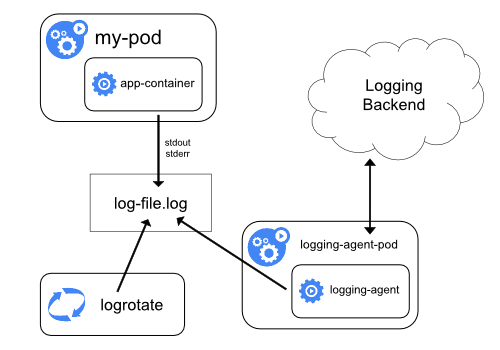
\includegraphics[scale=0.55]{img/3-background/kubernetes/node_agent.png}
    \caption{Using a node logging agent cluster-level logging. \protect\footnotemark}
    \label{fig:node_agent}
\end{figure}

\footnotetext{Source: https://kubernetes.io/images/docs/user-guide/logging/logging-with-node-agent.png (accessed 10.03.2025)}

\section{Centralized Logging Solution}

\subsection{Architecture}
%which centralized logging solution? Yours?
The centralized logging solution comprises two applications:

\begin{enumerate}
    \item Logging Operator – Forwards logs from the Kubernetes cluster. 
    \item Graylog – Serves as the logging solution for storing, processing, and analyzing logs.
\end{enumerate}

\subsection{Logging Operator}

The Logging Operator \cite{logoperator} automates the deployment and configuration of a Kubernetes logging pipeline, simplifying log management. \textbf{FluentBit} acts as a node-level logging agent. Fluent Bit is deployed as a DaemonSet, meaning it is running on each node to collect container logs, enrich them with Kubernetes metadata, and forward them to a log forwarder \textbf{Fluentd}. The operator manages both log collectors and forwarders, as well as routing rules for log distribution.

The Logging Operator collects and aggregates logs, then forwards them to Graylog for centralized storage and analysis.

\begin{figure}[H]
        \centering
        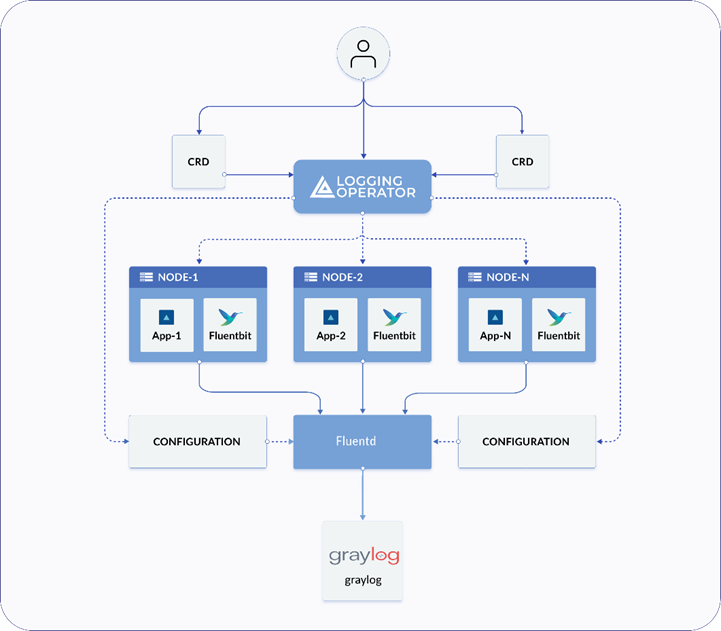
\includegraphics[]{img/3-background/centralized_logging/architecture.png}
        \caption{Centralized Logging Solution Architecture. \protect\footnotemark}
        \label{fig:centralized_logging_architecture}
\end{figure}

\footnotetext{Source: https://kube-logging.dev/docs/img/logging\_operator\_flow.png (adjusted) (accessed: 10.12.2024)}

\subsubsection{Configuration}

There are four main resources in the logging setup for Fluentd to configure: \textbf{Flow, Output, ClusterFlow, and ClusterOutput} \cite{logconfig}.  
\begin{itemize}
    \item \textbf{Flow:} Directs logs from applications within a specific namespace to designated outputs.
    \item \textbf{Output:} Defines a destination where Fluentd Flows can send log messages. Since it is a namespaced resource, only Flows within the same namespace can access it.
    \item \textbf{ClusterOutput:} Similar to Output but without namespace restrictions, allowing logs from multiple namespaces to be forwarded to a central destination.
    \item \textbf{ClusterFlow:} Functions like Flow but operates across all namespaces, enabling cluster-wide log forwarding.
\end{itemize}

%The Logging Operator can be installed on Kubernetes environments using Helm charts.
%this format is very messy here
%https://logging.paluch.biz/syslog-level-mapping.html
%https://docs.rs/gelf/latest/gelf/enum.Level.html

\subsubsection{Flow Configuration}

Flow defines a logging flow for Fluentd with filters and outputs. The Flow is a namespaced resource, so only logs from the same namespaces are collected. You can specify match statements to select or exclude logs according to Kubernetes labels, container and host names. Match statements are evaluated in order they are defined and processed only until the first matching select or exclude rule applies. A Flow consists of filters and outputs and only collects logs from the same namespace. Match statements allow filtering logs based on Kubernetes labels, container names, or host names. \cite{logconfig}

\subsubsection{Filtering and Processing Logs}

Additionally, you can define one or more filters within a Flow \cite{fluentdfilters}. Filters can perform various actions on the logs. A Flow can contain multiple filters, applied in sequence. These filters enable:

\begin{itemize}
    \item \textbf{Log enrichment} with additional data
    \item \textbf{Modification of log content}
    \item \textbf{Extraction of specific values} from log entries
\end{itemize}


\subsection{Rancher Logging App}

The Logging operator has also been integrated as Rancher's logging solution, replacing the previous in-house system. To enable logging for a Rancher-managed cluster, the "Logging" App from the Apps page in the Rancher \gls{ui} can be installed.

\begin{figure}[H]
        \centering
        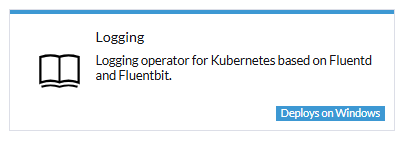
\includegraphics[]{img/3-background/centralized_logging/logging_app.png}
        \caption{Rancher Logging App.}
        \label{fig:logging_app}
\end{figure}

The key advantage of this deployment is the integrated Role-Based Access Control (RBAC). Rancher "Logging" App provides two roles: \texttt{logging-admin} and \texttt{logging-view}.
% do I understand correctly that those two roles can also be called Project Owners and Project Members? Maybe explain that

\begin{figure}[H]
        \centering
        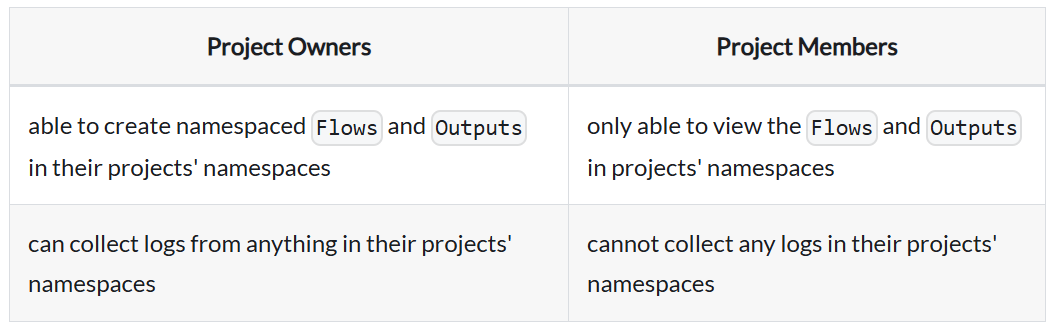
\includegraphics[scale=0.7]{img/3-background/rancher_logging_app/roles.png}
        \caption{Roles for Rancher "Logging". \protect\footnotemark}
        \label{fig:roles}
\end{figure}

\footnotetext{Source: https://ranchermanager.docs.rancher.com/integrations-in-rancher/logging/rbac-for-logging (accessed: 19.03.2025}

\section{Graylog}

Graylog is a centralized log management solution designed for log aggregation, analysis, and management. It was developed to address usability and cost challenges associated with existing log management platforms. It started in 2009 as an open-source project.

Graylog is an integrated tool where log messages are stored with Elasticsearch or OpenSearch, while associated metadata is stored in MongoDB. An application process serves as a central log server; a web interface can be used for querying and visualizing the data and for managing Graylog. A major advantage of Graylog is the ability to restrict access to the system. Graylog allows users to search, filter, and categorize log messages using configurable rules, and to set up dashboards. \cite{hopf2016elasticsearch}

Graylog Open is the free, open-source version of Graylog, providing core log management capabilities, including log data collection, enrichment, storage, and analysis. The development of Graylog Open is supported by community contributions. Graylog Open, licensed under \gls{sspl}, is a self-managed solution widely used by organizations and individuals for processing and analyzing log data. 

In addition to the open-source version, enterprise options are available for organizations requiring advanced security, compliance, and scalability features.

The Graylog Stack consists of:  

\begin{enumerate}
    \item{Graylog} - Responsible for log processing and visualization 
    \item{Data Node} – Handles storage and indexing
    \item{MongoDB} – Stores metadata and configuration
\end{enumerate} 

\begin{figure}[H]
    \centering
    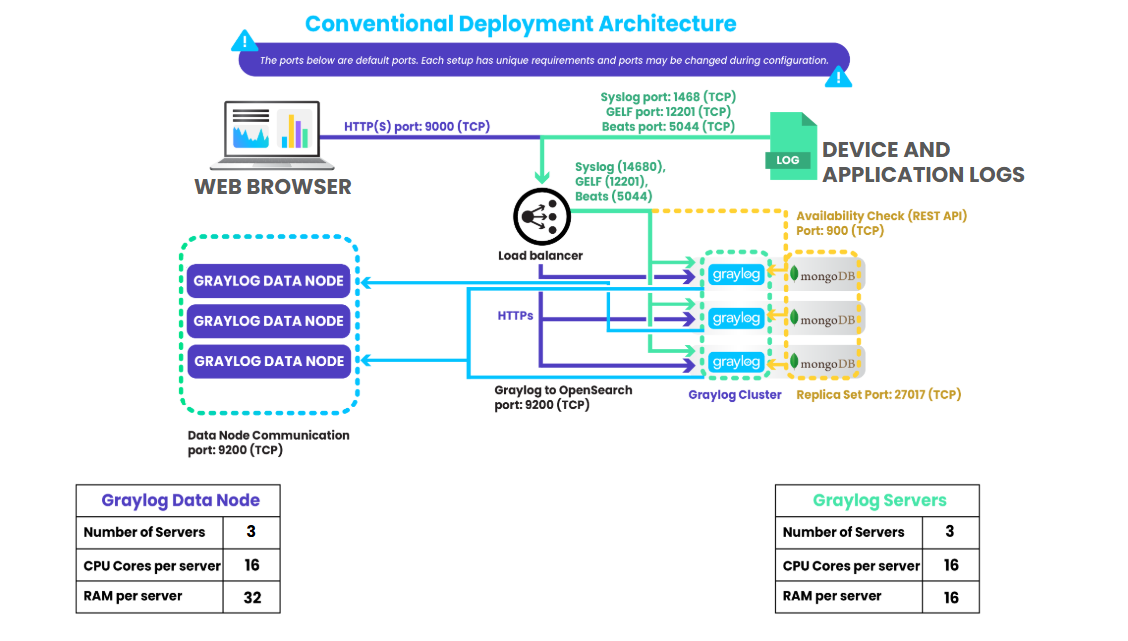
\includegraphics[scale=0.36]{img/3-background/graylog/deployment.png}
    \caption{Graylog Conventional Deployment. }
    \label{fig:graylog_deployment}
\end{figure}

\footnotetext{Source: https://go2docs.graylog.org/current/resources/images/graylog\_architecture/conventionaldeploymentarchitecture.png (accessed 10.03.2025)}

A Graylog Data Node manages ElasticSearch/OpenSearch, which provides indexing and search functionality.  

A conventional deployment is the recommended architecture for large-scale production environments, particularly those handling high log volumes or supporting multiple Graylog users. This setup distributes Graylog components across multiple nodes, ensuring high availability, scalability, and fault tolerance.  

The accompanying diagram \ref{fig:graylog_deployment} provides a visual representation of this architectural model, illustrating its components, data flow, resource allocation, hardware, and storage requirements.

\section{Kano Model}

Kano’s Model of Attractive Quality \cite{kano1984attractive} introduced in 1984, has become one of the most widely used quality models among researchers across various industries. It is a theory for understanding how different features of a product impact customer satisfaction. 

\begin{figure}[H]
        \centering
        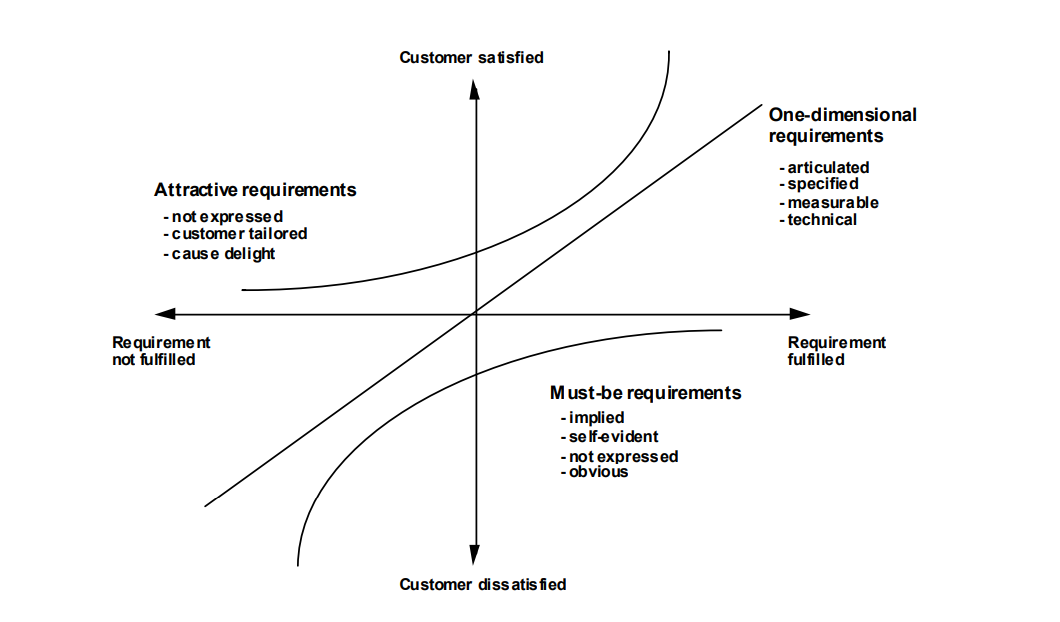
\includegraphics[scale=0.9]{img/3-background/kano/kano.png}
        \caption{Kano diagram. \cite{kanomodel1996}.}
        \label{fig:kano}
\end{figure}

The horizontal axis of the Kano diagram in Figure \ref{fig:kano} indicates how fully functional some aspect of a product is, and the vertical axis indicates how satisfied the customer is. Indifference would be plotted on \ref{fig:kano} roughly along the horizontal axis, meaning that the customer is neither satisfied nor dissatisfied. The line going through the origin at 45 degrees shows the situation in which customer satisfaction is simply proportional to whether requirement is full filled. They are defined as “One-dimensional” customer requirements. Curves are labeled as "Must-be" and "Attractive" requirements. The "Must-be" curve indicates aspects where the customer is more dissatisfied when the product is less functional, but where the customer’s satisfaction never rises above neutral no matter how functional the product becomes. The "Attractive" curve indicates areas in which 
the customer is more satisfied when the product is more functional but is not dissatisfied when the product is less functional. \cite{berger1993kano}

The Kano model uses a structured questionnaire to classify such "One-dimensional", "Attractive", "Must-be", and "Indifferent" customer requirements quality attributes of a product or service. Each attribute is assessed through two paired questions: the \textbf{functional question}, which asks about the consumer’s reaction when the attribute is present, and the \textbf{dysfunctional question}, which asks their response when it is absent. The collected data is analyzed using a specialized evaluation table to categorize attributes for each respondent. The final classification is derived by examining the frequency of individual responses. \cite{kanomodel1996}

The Figure \ref{fig:kanomodel} illustrates an example of the questionnaire and the subsequent analysis workflow. Based on the responses to the two parts of the question in the figure, the product feature can be classified into one of six categories:

\begin{enumerate}
    \item[] A = Attractive 
    \item[] M = Must-be 
    \item[] O = One-dimensional 
    \item[] I = Indifferent 
    \item[] R = Reverse
    \item[] Q = Questionable 
\end{enumerate}

"R" and "Q" categories indicate the following situations: 

There is a contradiction in the customer’s answers to the questions (= Questionable); or apriori judgment of functional and dysfunctional was the reverse what the customer feels (= Reverse). \cite{berger1993kano}

The figure \ref{fig:kanomodel} displays a functional and dysfunctional question at the top as an example from the questionnaire. In the middle, it presents the Kano evaluation table, and at the bottom, it shows the tabulation of responses for each customer requirement in a Kano questionnaire.

\begin{figure}[h]
        \centering
        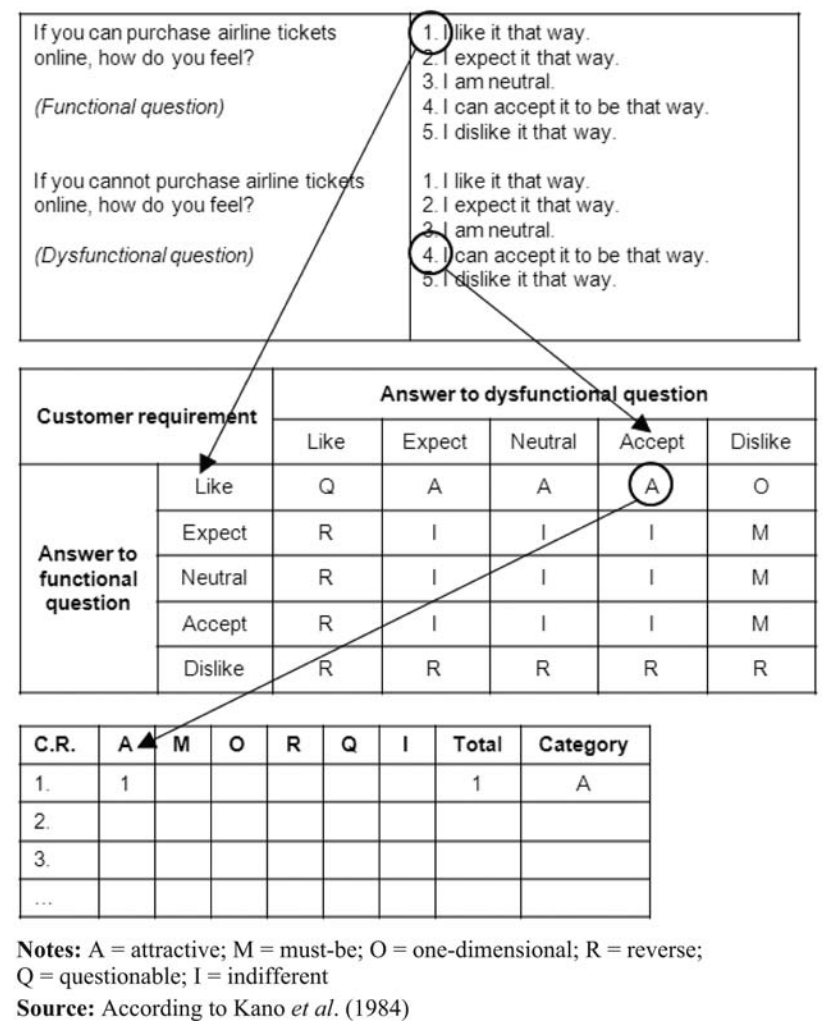
\includegraphics[scale=0.8]{img/3-background/kano/kanomodel.png}
        \caption{The Kano Method \cite{kanomodel1996}.}
        \label{fig:kanomodel}
\end{figure}

\clearpage
\textbf{Analyzing the Results}

Different approaches to classifying features using the Kano model can lead to varying outcomes. Mikulic and Prebežac \cite{mikulic2011} recommend that, instead of relying solely on one approach, these methods should be viewed as complementary, as each offers unique insights rather than serving as interchangeable alternatives. 

\textbf{Simple method}

The easiest method is evaluation and interpretation according to the frequency of answers. A simple way to rank the requirements is to score each according to the mode (the most frequently occurring dimension) in each row of the tabulation matrix. One can also look at the second most frequent dimension for each requirement. \cite{berger1993kano}

For example, if a feature is categorized as "R" (Reverse) once, "A" (Attractive) three times, and "I" (Indifferent ) twice, the category with the most votes is Attractive. Therefore, the feature is classified as a "A" overall.

\textbf{Continuous scale}

Each response is first converted onto a numerical scale, with more weight attached to positive end of the scale. The asymmetrical scale is used so that "M" (Must-be) and "O" (One-dimensional) are stronger responses than "R" (Reverse) or "Q" (Questionable). The "R" (Reverse) type responses are given less weight by being pulled toward zero. Less weight is given to the less strong responses to diminish their influence on the average. \cite{berger1993kano} 

\begin{table}[H]
    \centering
    \begin{tabular}{lccccc}
        \hline
        & Dislike & Tolerate & Neutral & Expect & Like \\
        \hline
        Feature is present & -2 & -1 & 0 & 2 & 4 \\
        Feature is absent  & 4  & 2  & 0 & -1 & -2 \\
        \hline
    \end{tabular}
    \caption{Kano Model Evaluation Table}
    \label{tab:kano}
\end{table}

The responses to questions are plotted as points in a two-dimensional coordinate system. The most distinct or representative points for each Kano category within this system are defined as follows:  

\begin{itemize}
    \item[] Reverse: (X = -2, Y = -2)
    \item[] Indifferent: (X = 0, Y = 0)
    \item[] One-dimensional: (X = 4, Y = 4)
    \item[] Must-be: (X = 4, Y = 0)
    \item[] Attractive: (X = 0, Y = 4)
\end{itemize}

For evaluation, all responses are averaged together which results in a pair of numbers X and Y (one for functional, one for dysfunctional). This pair represents the aggregate total of all the different opinions of the participants. The pairs for all features are plotted onto a grid, with the different areas of the grid mapped out to Kano categories. The averages should mostly fall in the range 0 to 4, since negative values are either Questionable or Reverse. These points are highlighted with underlining and bold text in Figure \ref{fig:analysis}. All other XY point combinations appear as interpolations between these specific points. \cite{berger1993kano}

\begin{figure}[H]
        \centering
        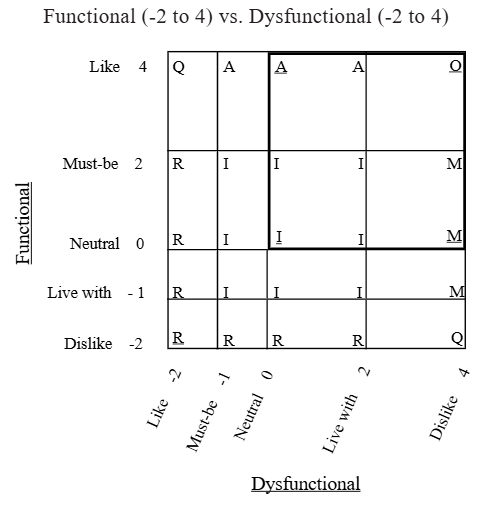
\includegraphics[scale=1]{img/3-background/kano/analysis.png}
        \caption{Continuous scale grid. \cite{berger1993kano}.}
        \label{fig:analysis}
\end{figure}

\textbf{Customer satisfaction coefficient}

Customer satisfaction coefficient (CS coefficient) analysis is a way of getting an overall estimate of how customer satisfaction would change on an absolute scale, if the feature were present or not. The data is reduced to two numbers called "Better" and "Worse", which will be calculated as follows: \cite{timko1993}

\begin{equation}
    \text{Better} = \frac{A + O}{A + O + M + I}
\end{equation}

\begin{equation}
    \text{Worse} = - \frac{O + M }{A + O + M + I}
\end{equation}

Total = (Attractive (A) + One-dimensional (O) + Must\_have (M) + Indifferent (I))

Better = ((Attractive (A) + One-dimensional (O)) / Total

Worse = ((One-dimensional (O) + Must\_have (M)) / Total) * -1

The "Better" number indicates how much customer satisfaction is increased if a feature is provided (score increased by this positive number) and "Worse" indicates how much customer satisfaction is decreased if the feature is not (score decreased by this number). Pairs of Better and Worse points for each customer requirement can be plotted on a two-dimensional graph.

\begin{figure}[H]
        \centering
        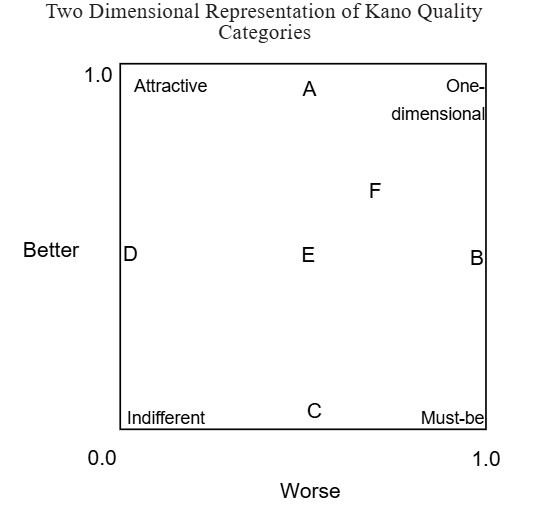
\includegraphics[]{img/3-background/kano/2dkano.png}
        \caption{ \cite{berger1993kano}.}
        \label{fig:2dkano}
\end{figure}

The Figure \cite{fig:2dkano} shows the scale for CS coefficient analysis, where "Better" runs from 
0.0 to 1.0 up the vertical axis, and "Worse" runs from 0.0 to 1.0 along the horizontal axis. The minus sign has been left off Worse on this graph.

\section{Company's Infrastructure}

The company's resources will be utilized for evaluation. A separate test Kubernetes cluster within the company's infrastructure was used for evaluation, followed by integration of the solution into productive cluster.
The logs will be analyzed with the company's consent.

Two RKE1 clusters are deployed on the company's infrastructure were used:

\begin{enumerate}
    \item[] \texttt{testcluster} 
    
    A test cluster: Kubernetes v1.28.10 Amd64, 12 cores, 47 GiB, 3 Nodes
    \item[] \texttt{devops} 
    
    A productive cluster: Kubernetes v1.26.15 Amd64, 72 cores, 533Gib, 18 Nodes
\end{enumerate}

Since 2020, the deployment of internal applications has transitioned to Helm Charts \cite{helm} wherever possible. Helm Charts enable the pre-configured provisioning of all components, allowing applications to be installed in Kubernetes with a single click. Once created, the Helm Chart is be uploaded to the company's local Git repository, which Rancher checks every five minutes to update the application directory accordingly.

\section{Application Log Management at the Company}

Since the company consists of many different teams, each with its own customers and software needs, the current situation regarding log management will be explained by use cases from the internal Kubernetes cluster.  

The following use cases illustrate their current state of logging, future expectations, and requirements for the logging solution. These observations are made by interviewing the individuals responsible for the respective applications. 

Four use cases will be presented: GitLab, SKPBO, Rezert, and CLD \& METAPlus. These use cases represent three internally developed applications and one third-party application (GitLab).

\subsection{Use Case: Gitlab}

GitLab is a web-based platform for version control and collaboration on software projects. It is based on Git and offers features such as repository management, Continuous Integration (CI), Continuous Delivery (CD), code review, and issue tracking. \cite{gitlab}

A GitLab instance is used by the company internally, running on a productive Kubernetes cluster. In 2022, the central internal GitLab repository was migrated to the Kubernetes infrastructure. There is a test and a productive instance running on the cluster. For internal productive applications, there is a functional application manager and a technical application manager. An employee interviewed is registered as the technical application manager for GitLab.

\subsubsection{Current State}

The internal GitLab instance is running productively on the Kubernetes cluster. There are two namespaces: one for the test instance and one for the productive GitLab instance. 

Updates are first carried out in the test namespace. If successful, the productive instance is then updated. Various unusual errors have occurred in GitLab in the past, the origins of which were unclear. To further illustrate the current state, a scenario describing an issue in a production GitLab application is presented. \\

\textit{Scenario: Error in a production GitLab Application}

\begin{enumerate}
    \item Reporting the Issue: 
    
    An employee noticed a software malfunction and reported it to the technical application manager.
    
    \item Inspection of GitLab Components: 
    
    The manager inspects the software, verifies the malfunction, and proceeds to examine running pods individually (Figure \ref{fig:gitlab}).
    
    \begin{figure}[H]
        \centering
        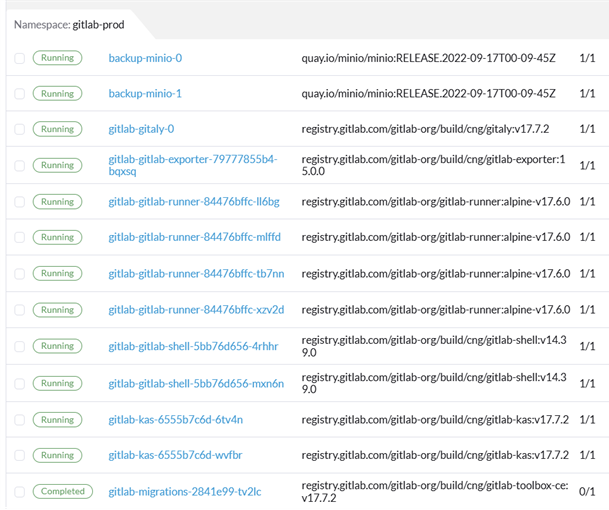
\includegraphics[]{img/3-background/gitlab/gitlab.png}
        \caption{Gitlab pods view on Rancher.}
        \label{fig:gitlab}
    \end{figure}
    
    \item Log Analysis: 
    
    The responsible person begins by searching for errors using the Rancher \gls{ui}. However, the search function in Rancher often malfunctions. Alternatively, logs can be downloaded manually from the Rancher \gls{ui} (\texttt{"Download"} button) or retrieved using the \texttt{"kubectl logs"} command. The downloaded logs only include data starting from the container’s initial launch. However, this approach comes with the drawback of discarding potentially valuable historical data that might be useful for diagnosing long-term or recurring issues. Since there is no backup mechanism currently in place, logs are lost after container restarts, and no history is saved.

    \begin{figure}[H]
        \centering
        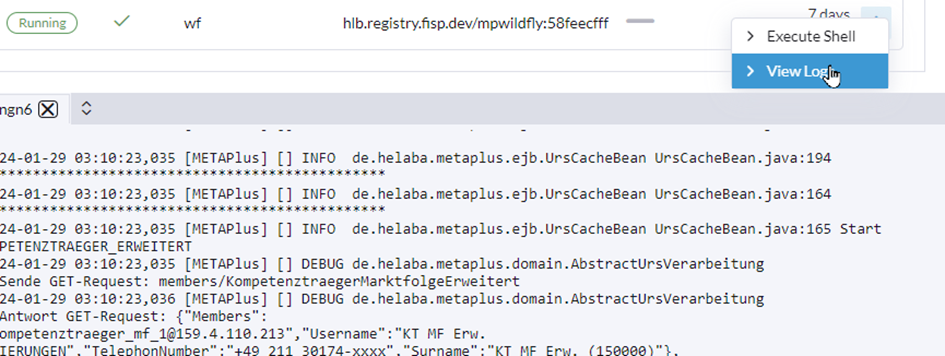
\includegraphics[scale=0.8]{img/3-background/gitlab/rancher_logs_gui.png}
        \caption{Gitlab Rancher GUI logs view.}
        \label{fig:rancher_logs_gui}
    \end{figure}

    \item Findings: 
    
    The person responsible was often unable to find any relevant log entries or errors, as the available logs either lacked useful information (such as irrelevant \texttt{"Timeout"} or \texttt{"Merge conflict"} errors). As a result, the workflow did not contribute to identifying or resolving the issue. Due to the overwhelming volume of logs and the need to inspect each pod’s logs separately, it was likely that critical errors went unnoticed, as there was no way to view the entire timeline in a consolidated manner.

    \item Resolution
    
    The only effective solution in such cases is to redeploy the application.
    
\end{enumerate}

At present, effective log analysis is not feasible. The sheer volume of data makes manual analysis impractical, while automated methods (e.g., using grep or writing Python script) demand significant effort to identify relevant information, for which there is neither the time nor the inclination. Consequently, the current solution is to redeploy the whole application, with the hope that the issue will be resolved through the restart process.

\subsubsection{Challenges \& Requirements}

\begin{enumerate}
    \item[-] GitLab test and production instances have approximately 20 pods running. Merging logs from different pods in chronological order is necessary.
    
    \item[-] Identify and eliminate recurring issues, which are unrelated to GitLab but still impact its functionality (e.g., a recurring request to an unavailable service).
    
    \item[-] Possibility of quick search: GitLab generates a large number of log messages. It should be possible to quickly search for specific entries, such as error logs.
    
    \item[-] Searching for specific values: e.g., filtering by a specific user or project. Extracting values as separate attributes to identify all logs relevant to the user or project that reported an error.
    
    \item[-] Alerts for critical errors: GitLab logs many errors that are not relevant to administrators (e.g., a Git merge request failing due to a merge conflict). Such errors should be ignored.
    
    \item[-] \gls{ad} user management is desirable to avoid manually creating user accounts for application managers.
\end{enumerate}

\subsection{Use Case: SKPBO}

The company's internal Kubernetes cluster serves as a test environment for development and test of SKPBO applications. It is not yet running productively in a containerized manner due to regulatory and technical reasons; however, the transition to a containerized production environment is in planning. The internal Kubernetes cluster runs in our own data center, providing greater flexibility and reducing management and administrative overhead. However, the productive instance runs on the infrastructure of a sister company, which is regulated by a contract with the customer. Since the provisioning and management of the production infrastructure are handled entirely by a sister company, the transition to containerized technologies often takes a long time.

SKPBO is a project that includes 5 different business applications accessible via a web browser. All requests pass through the Keycloak Identity Provider, which integrates multiple authentication mechanisms, permissions, and role management from other internal systems.

Keycloak is an open-source solution that provides a unified interface, abstracting and standardizing access to various business applications. The primary users are employees of a large bank. After authentication, they are directed to the business applications, which are developed internally using Java Spring Boot.

\subsubsection{Current State}

\textbf{Development/Test Environment (Kubernetes Cluster)}

The Kubernetes cluster is managed internally running on company's data center. Keycloak and Spring Boot applications run in their respective namespaces and communicate with each other. No centralized logging is in place. The internal Kubernetes environment is used for development and testing to prepare for a future transition to the production environment.

\textbf{Production Environment (Linux Servers)}

The production infrastructure is managed by a sister company.Applications run in production on Linux servers, where Spring Boot applications are manually started and managed. No centralized logging in place, logs are stored directly on the servers and only reviewed manually in case of incidents. The sister company offers Splunk as a centralized logging solution, but the team has not yet requested it.

\subsubsection{Challenges \& Requirements}

\begin{enumerate}
    \item[-] Aggregate logs from multiple instances centrally. Previously, there was only one Keycloak instance, so manual log searches were manageable. Multiple instances of Keycloak are planned to be used in the future, making manual log analysis significantly more complex.

    \item[-] Targeted Search \& Alerting
    
    Filter logs based on specific criteria (e.g., level=error).
    
    Set up automatic alerts for critical log entries.

    \item[-] OpenID Connect (OIDC) for Authentication

    Integration with Keycloak to allow external administrators to access logs without manually creating user accounts.

    \item[-] Efficient Storage Management
    
    Since the infrastructure is managed by the sister company, storage space is limited. Currently, logging is kept to a minimum to prevent the file system from filling up. Proposed idea: Send logs to Graylog and automatically delete them from servers to save storage space.

    \item[-] Access Control \& Data Protection

    A centralized access control model is needed. A Graylog administrator should be assigned to manage log streams in production. Logs contain sensitive/private information, so access rights must be clearly defined.

    \item[-] Expansion into a Comprehensive Monitoring Solution

    Extend beyond logging to capture additional system metrics.
    
    \item[-] Log Filtering \& Downloading
    
    Enable filtering and downloading of logs to facilitate easy sharing when needed.

    \item[-] Installation

    A possibility to deploy Graylog not only on a cluster but also directly on a server if the team decides to use it before transitioning to Kubernetes.

\end{enumerate}

\subsection{Use Case: CLD \& METAPlus}

Credit Loss Database (CLD)

The CLD is the central system for processing, calculating, and storing risk provisions for the bank's defaulted transactions.

METAPlus

The tool is used in the creditworthiness-driven savings bank lending business for new transactions. It is used for covenant monitoring and enables the processing of credit monitoring templates as well as other templates within a fully electronic workflow.
The primary users are employees of a large bank.

\subsubsection{Current State}

\textbf{Development/Test Environment (Kubernetes Cluster)}

The Kubernetes cluster is managed internally, running on company's data center. In the Kubernetes cluster every GitLab push automatically triggers a CLD/METAPlus release, including WildFly and a database server. No centralized logging is in place. The internal Kubernetes environment is used for development and testing to prepare for a future transition to the production environment.

\textbf{Production Environment}

Applications run productively at the customer’s site. The customer fully manages operations. However, in the case of major incidents where the bank cannot resolve the issue, the customer reaches out to the team and sends logs via E-mail.

\subsubsection{Challenges \& Requirements}

Since the instances on the Kubernetes cluster are only used to simplify the development process by automatically building and deploying branches for testing, the team lead does not see the need for a centralized logging solution. As they do not manage production, he believes that checking logs directly in the IDE during development is sufficient and that using a logging solution would not bring significant benefits.

Historically, when containers weren’t updated for extended periods, log files within them could grow significantly, leading to excessive memory usage in the pod. To mitigate this, log-rolling mechanisms (e.g., via libraries like Log4j) were implemented. These mechanisms automatically delete logs after they reach a certain size or age.

For in-house developed applications, it is possible to view logs through the Kubernetes plugin in IntelliJ or other IDEs. This eliminates the need to manually retrieve logs via the Rancher GUI or command line. 

Option 1: Via the Rancher interface:

\begin{figure}[H]
        \centering
        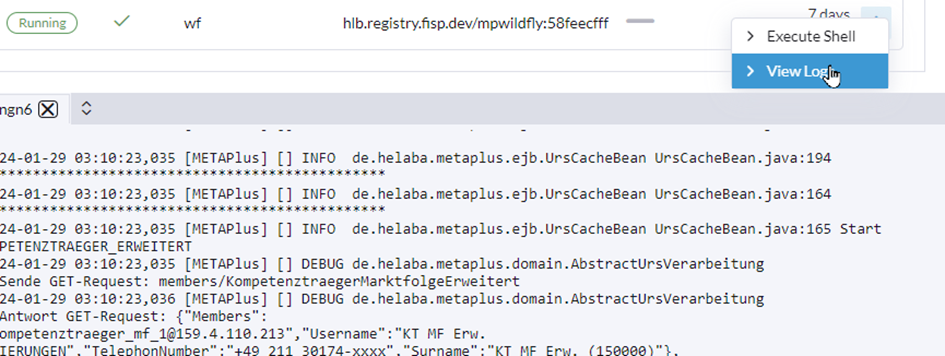
\includegraphics[scale=0.8]{img/3-background/gitlab/rancher_logs_gui.png}
        \caption{}
        \label{fig:rancher_logs_gui}
    \end{figure}

Option 2: Via the Kubernetes plugin in IntelliJ

\begin{figure}[H]
        \centering
        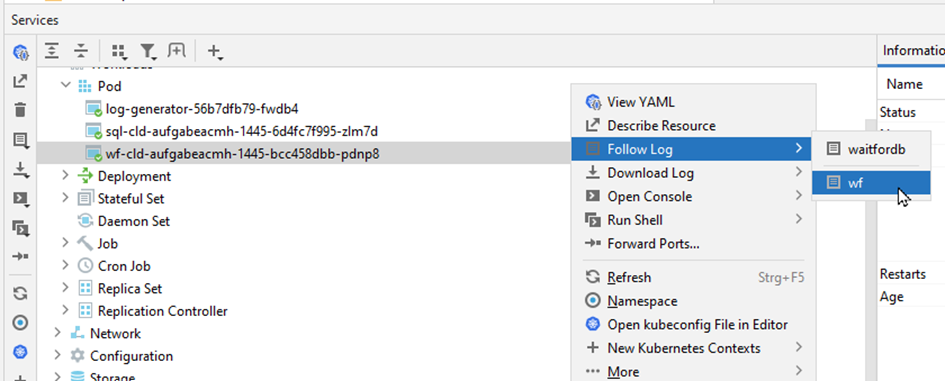
\includegraphics[scale=0.8]{img/3-background/gitlab/logs_plugin.png}
        \caption{}
        \label{fig:logs_plugin}
    \end{figure}

\subsection{UseCase: Rezert Tool}

An application „Rezert Tool“ was developed for internal use that significantly simplifies the recertification process by automatically processing data from the respective systems into tailored tickets containing all necessary information. As a result, 90\% of recertifications can be completed simply by closing the ticket.
The DevOps Rezert Tool is implemented using microservices based on Kubernetes and Kafka.

\subsubsection{Current State}

The development instance is running productively on one cluster, and the productive instance on the other cluster.

\subsubsection{Challenges \& Requirements}

\begin{enumerate}
    \item[-] Since one process goes through all microservices, we need logs from all of them to trace the entire workflow. Logs need to be combined from different microservices in chronological order.
    \item[-] Quickly access logs in case of incidents.
    \item[-] Search by process: find the process ID field and display logs from different microservices. It is neccesary to identify in which service did an error occur.
    \item[-] Alerts for errors.
    \item[-] Dashboard request: display the entire process flow by process ID, showing logs from each service and whether it was successfully completed (e.g., from request to ticket creation = SUCCESS)
\end{enumerate}



\end{document}
